\documentclass{standalone}
\usepackage{pgfplots}
\usetikzlibrary{shapes.geometric, intersections, calc}
\pgfplotsset{compat=1.7}

\begin{document}
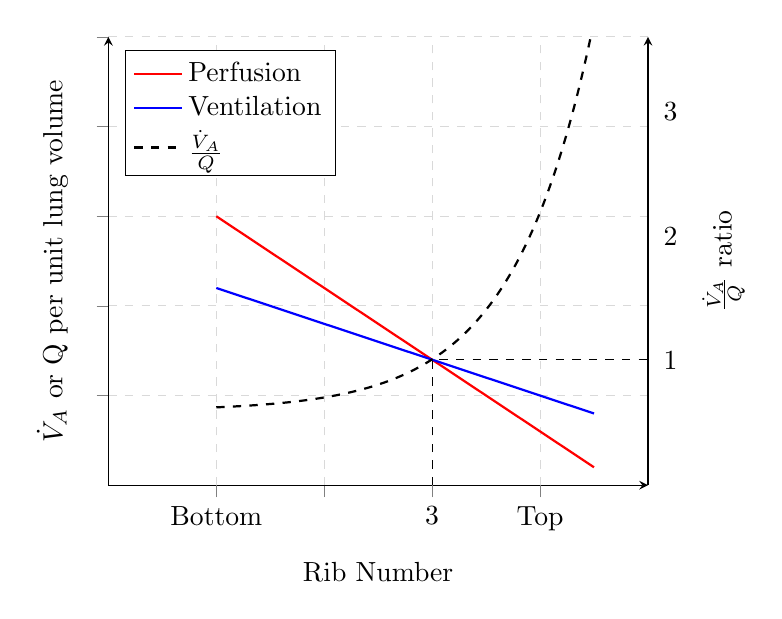
\begin{tikzpicture}
    \begin{axis}[
        axis x line=middle,
        axis y line=middle,
        grid = major,
        grid style={dashed, gray!30},
    	  x label style={at={(axis description cs:0.5,-0.1)},anchor=north},
	  y label style={at={(axis description cs:-0.1,.5)},rotate=90,anchor=south,precision=2},
	  xticklabels={},
	yticklabels={},
	extra x ticks={1, 3, 4},
extra x tick labels = {Bottom, 3, Top},
        xmin=0,
        xmax= 5,
        ymin= 0,
        ymax= 5,
	 ylabel near ticks,
	xlabel near ticks,
        xlabel=Rib Number,
        ylabel=$\dot{V}_A$ or Q per unit lung volume,
        tick align=outside,
legend pos = north west,
legend cell align={left}]

	\coordinate (o) (0,0);
	\addplot[domain=1:4.5, red, thick,samples=500] {3.8 - 0.8*x};
\addlegendentry{Perfusion};
	\addplot[domain=1:4.5, blue, thick,samples=500] {2.6 - 0.4*x};
\addlegendentry{Ventilation};
	\addplot[domain=1:4.5, black, dashed, thick,samples=500] {0.01*e^(1.35*x) +0.83};
    \addlegendentry{$\frac{\dot{V}_A}{Q}$}
	\draw [black, thin, dashed] (300,0) -- (300,140) -- (500, 140);
\end{axis}
     \begin{axis}[
       xmin=0,xmax=2,ymin=0.4,ymax=4,
       axis x line=none,
 	axis y line=right,
       yticklabels={},
ytick style={draw=none},
	extra y ticks={1.4,2.4,3.4},
extra y tick labels = {1,2,3},
       ylabel near ticks,
       ylabel={$\frac{\dot{V}_A}{Q}$ ratio}
     ]
     \end{axis}



\end{tikzpicture} 
\end{document}